% !TEX TS-program = pdflatex
% !TEX encoding = UTF-8 Unicode

%************************************************
\chapter{L'opera Sp.I.R.E}
\label{chp:L'opera Sp.I.R.E}
%************************************************

	\begin{flushright}
		\textit{[...] bello come la retrattilità degli artigli degli uccelli rapaci; o ancora, come l'incertezza dei movimenti muscolari nelle pieghe delle parti molli della regione cervicale posteriore; [...] e soprattutto, come l'incontro fortuito su un tavolo di dissezione di una macchina da cucire e di un ombrello!
		Isidore Lucien Ducasse}
	\end{flushright}

Tutto ebbe inizio nel luglio del 2017.

Nel corso della manifestazione \textit{ArteScienza 2017} tenutasi al Goethe Institute, venne eseguita una composizione di Pierre Jodlowski: \textit{Ombra della Mente}, ispirata ad alcuni scritti di Alda Merini. Il lavoro del compositore francese era diviso tra una parte teatrale recitata e una parte musicale, entrambe eseguite da una clarinettista e da una soprano. La fusione tra momenti prettamente teatrali e parti musicali ebbero un effetto tagliente sulla mia produzione musicale. Ogni intervento recitante era contrappuntato da rumori prodotti tramite lo strofinio di una matita su un foglio di carta e la frizione di una piccola molla presente nella meccanica della lampada di scena. Il tutto era elaborato in live electronics. L'effetto della molla sfregata e amplificata da un microfono a contatto, mi fece riaffiorare alla mente molti concerti di musica underground seguiti in passato (l'utilizzo delle molle, oltre ad appartenere all'universo della musica colta è stato abusato in ambienti musicali \textit{noise}\footnote{genere che utilizza il rumore come base principale per creare delle composizioni} e di musica cosiddetta "industriale" (chiamata così, proprio per sottolineare l'utilizzo di materiale di scarto di industrie e fabbriche).

\begin{small}
\begin{quotation}
[...] still the noise in the mind: that's it's the first task - then everything else will follow in time\footnote{R. Murray Schafer, \textit{The tuning of the world}, Alfred A. Knopf, New York 1977 \\}.
\end{quotation}
\end{small}

Andando avanti negli studi notai che, già negli anni '50 del Novecento, John Cage cercò di far percepire, tramite l'amplificazione con elettromagneti e microfoni a contatti, i suoni non udibili\footnote{qui faccio riferimento a \textit{Cartridge Music}}. Durante il corso di \textit{Interpretazione del repertorio della musica elettroacustica} del Mº Giuseppe Silvi ripercorremmo tutto lo scenario cagiano e iniziai, così, ad interessarmi in modo più accurato all'universo delle molle e alle loro particolarità timbriche.

\begin{small}
\begin{quotation}
Si può dire che la musica moderna in generale è stata la storia della liberazione della dissonanza, così la nuova musica è parte del tentativo di liberare tutti i suoni udibili dalle limitazioni del pregiudizio musicale.
Un singolo suono in sé non è né musicale né non musicale; è semplicemente suono. [...]

La musica mi sembrava ora l'organizzazione del suono, l'organizzazione di qualunque suono ottenuto con qualunque mezzo\footnote{John Cage, \textit{Confessioni di un compositore} in AA.VV. (a cura di G. Bonomo e G. Furghieri), \textit{Riga n. 15} - John Cage, Milano, Marcos y Marcos, Milano 1998}.
\end{quotation}
\end{small}

Dalle parole di Cage emerge una sostanziale verità, ovvero, tocca al compositore trasformare un suono in qualcosa di musicale, legando ad un andamento formale adeguato. 

Iniziai così le ricerche sia sui materiali e gli oggetti sonori che su forme musicali vicine allo scenario contemporaneo. Fortuito fu il lavoro assieme al Mº Michelangelo Lupone al Centro di Ricerche Musicali (CRM) sito in Roma. Per tutta l'estate del 2017 gli feci da assistente per la creazione di un'installazione ideata in collaborazione con l'artista Licia Galizia. L'opera in questione era la scenografia interattiva dello spettacolo coreutico \textit{Corpus 2.0}. Il lavoro consisteva nell'applicare all'interno dell'installazione, vari diffusori e piezoelettrici che servivano rispettivamente per la diffusione sonora e l'interazione con i danzatori. L'utilizzo di specifici altoparlanti e il controllo di parametri tramite il tocco, mi fece avvicinare ad un mondo a me limitrofo ma ancora in parte sconosciuto: quello dell'interazione tra uomo e macchina.

%************************************************

\section{Necessità di uno strumento dedicato}

\begin{small}
\begin{quotation}
Lo strumento musicale è il risultato di un insieme complesso di condizioni culturali.

Le sue caratteristiche tecnologiche e la sua \textit{structura} di oggetto composto, devono consentire la rappresentazione di un determinato linguaggio musicale, caratterizzato da aspetti estetici, espressivi e stilistici che implicano una prassi esecutiva consolidata, o almeno condivisa in un determinato contesto\footnote{Silvia Lanzalone Strumenti aumentati in Acustica UTET}.
\end{quotation}
\end{small}

La creazione di uno strumento musicale, quindi, comportava molte problematiche soprattutto a livello stilistico e di concetto. 

\begin{small}
\begin{quotation}
La ricerca di una definizione ontologica della musica è quindi strettamente connessa alla definizione dei confini tra un semplice oggetto che produce suono e uno strumento musicale, la cui prerogativa non può prescindere dal riconoscimento di un suo ruolo funzionale o simbolico in una data società\footnote{\textit{ibidem}}.
\end{quotation}
\end{small}

La linea di confine tra uno strumento musicale e un oggetto che produce suono è strettamente legata al suo utilizzo. Basandomi su queste nozioni, mi presi del tempo per far sedimentare in me delle nuove idee. Le giornate di lavoro al CRM diventarono fonte di suggestioni sull'utilizzo di oggetti risonanti e sulle loro capacità timbriche. Ogni oggetto sonoro diventò frutto di studio, anche minimo a volte, per via dei tempi brevi dati dalle consegne. Questo fu l'universo sonoro al quale mi aggrappai per la fascinazione che suscitava in me.

Giorno per giorno si andava a materializzare un'idea sempre più nitida, fino al giorno del mio esame del III anno di composizione elettroacustica.

Un esercizio, un brano, un piccolo studio sulle armoniche del pianoforte. La composizione partiva dalla trasformazione di un gesto sonoro: il pedale di risonanza in \textit{\textbf{fff}} seguito da cellule sonore inarmoniche composte da cluster e piccole volatine. I Gesti venivano elaborati tramite tre convoluzioni. Ogni convolutore apparteneva ad un universo sonoro a sé:

\begin{itemize}
\item{la prima convoluzione era la stessa cassa di risonanza del pianoforte eccitata dal pedale di risonanza calcato in \textit{\textbf{fff}};}
\item{la seconda convoluzione era creata registrando la molla della stessa lampada da tavolo utilizzata da Pierre Jodlowski;}
\item{la terza convoluzione era un'eccitazione del manico di una chitarra elettrica su un amplificatore a transistor.}
\end{itemize}

%\begin{floatingfigure}{10cm}
%\mbox{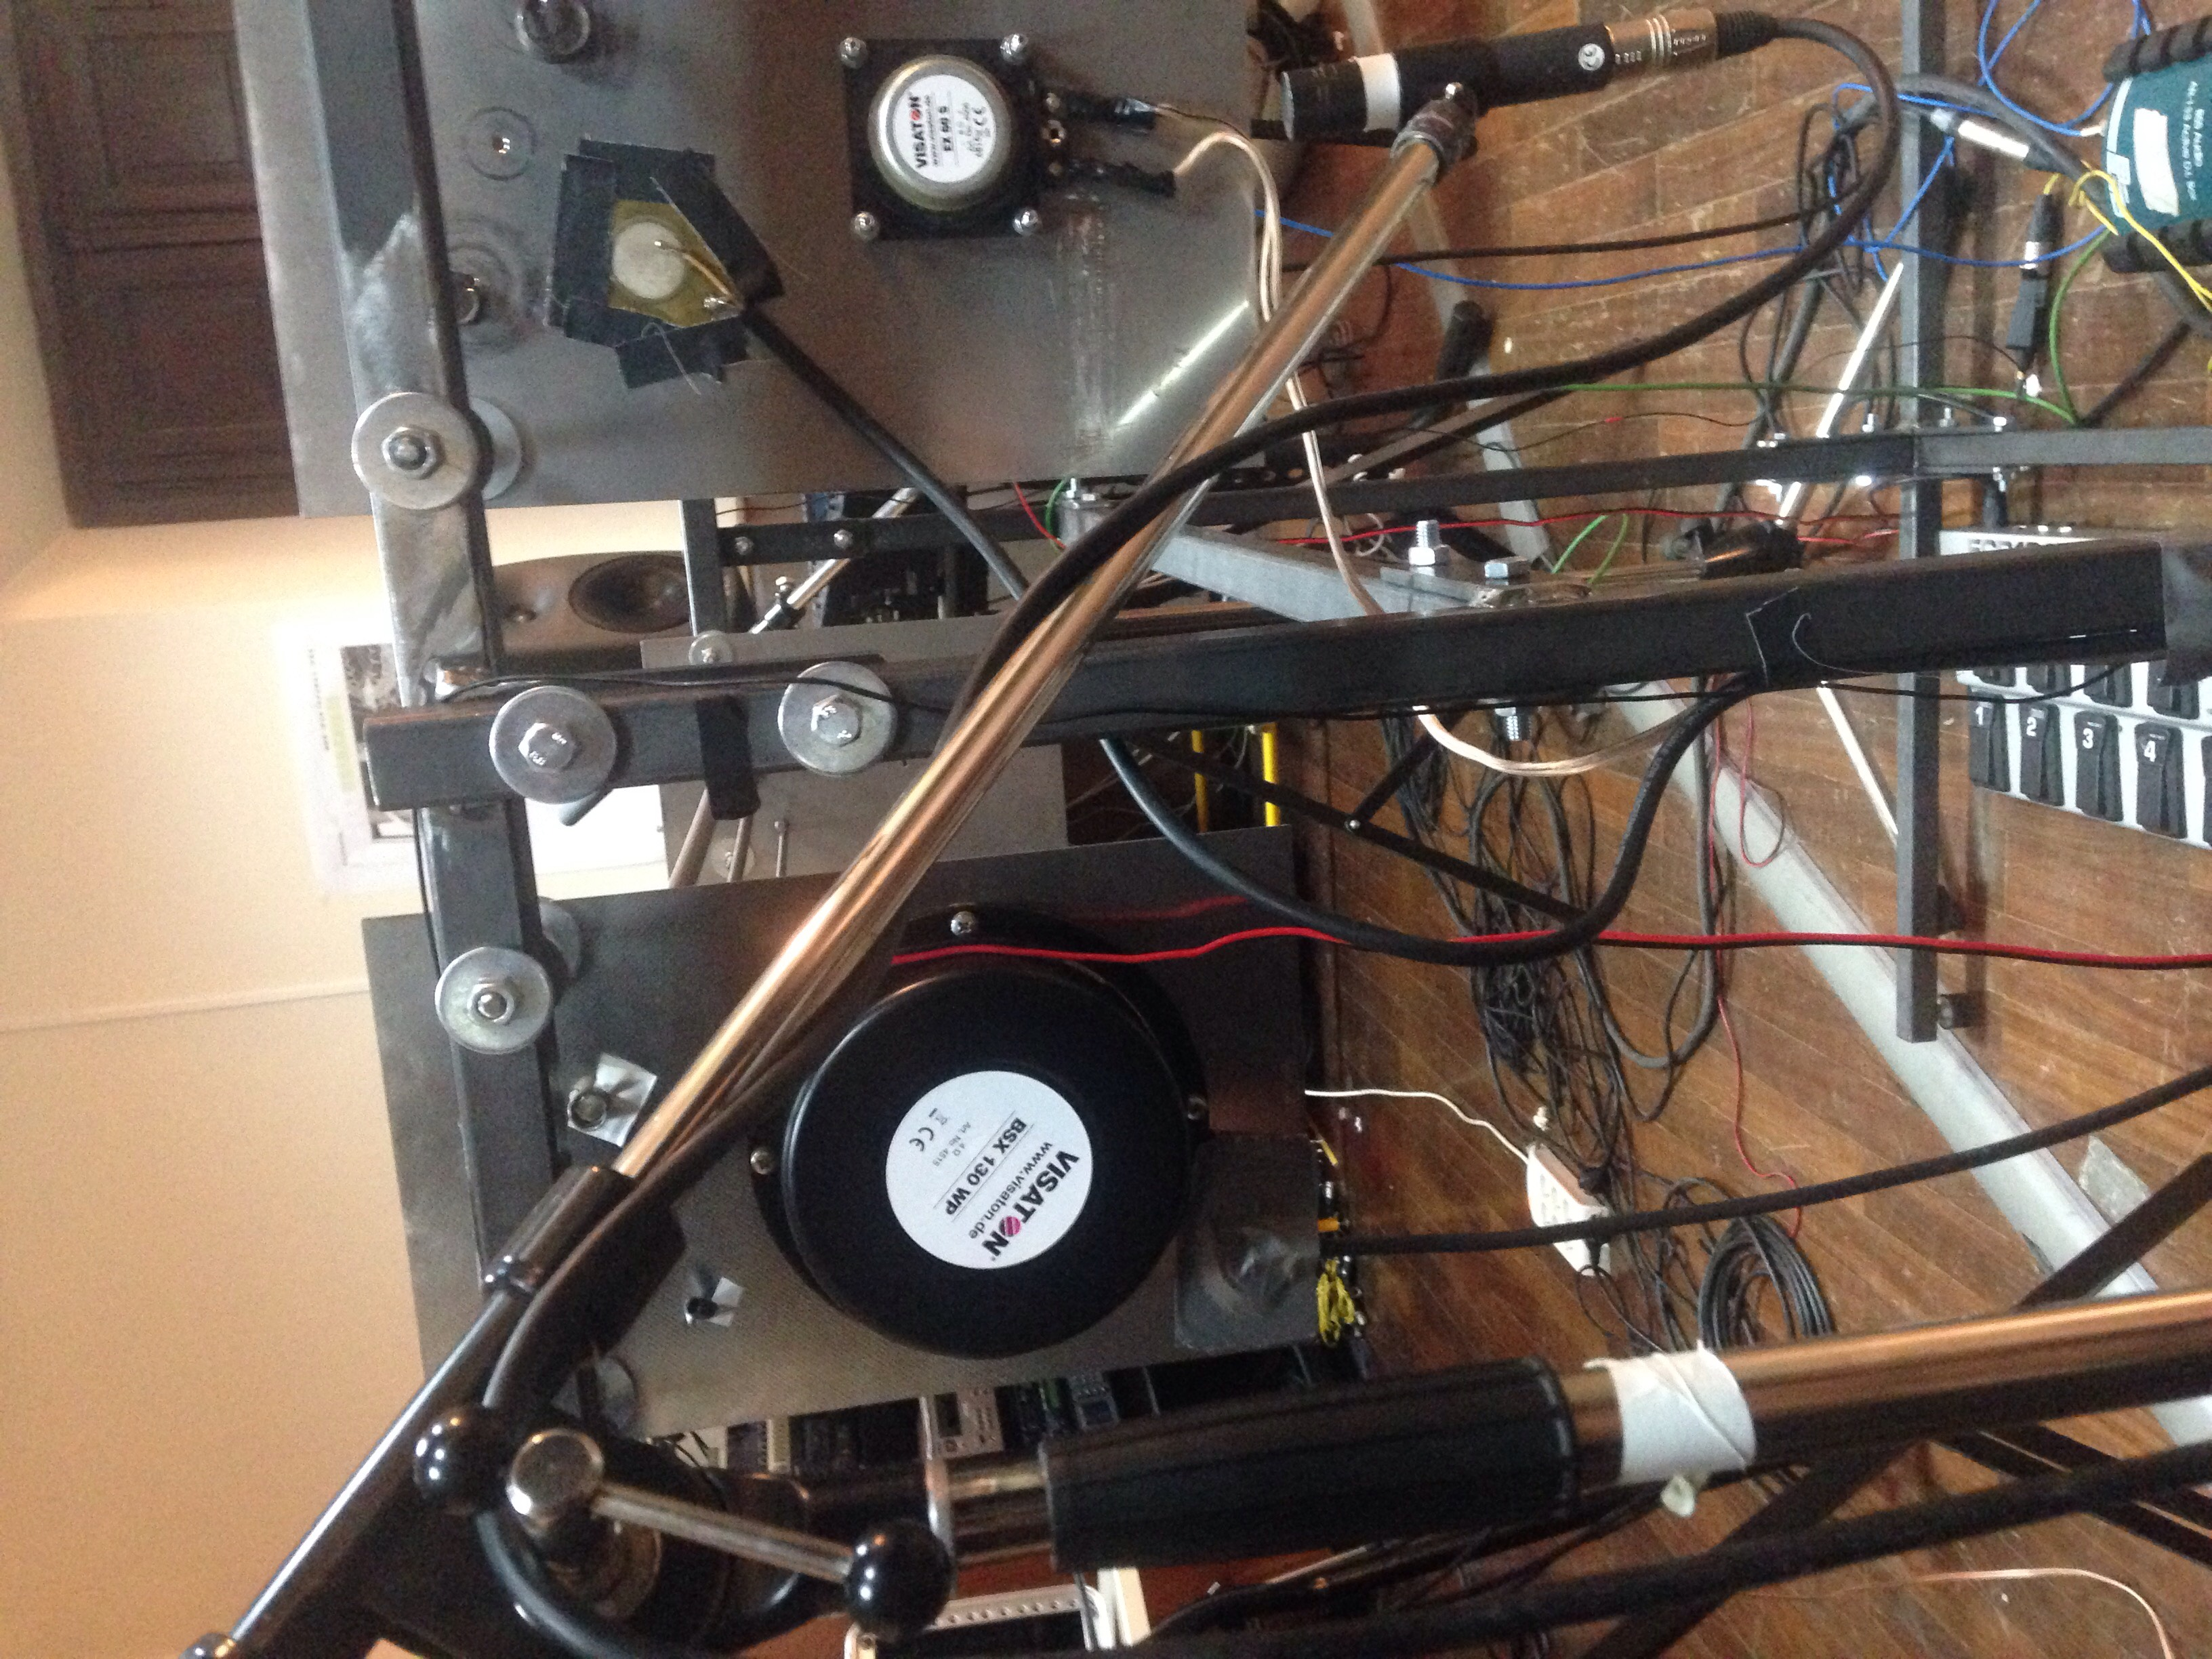
\epsfig{file=Spire1.jpg,width=8cm}}
%\small{\caption{\textit{particolare attuatori}}}
%\end{floatingfigure}
%

I risultati delle convoluzioni erano affascinanti, ma non mi soddisfacevano,  era come se volessi creare un convolutore che potesse essere, in qualche modo, anche un gesto scenico. Da qui alla creazione del mio iper-strumento, il passo fu breve. Riuscii finalmente ad avere del tempo per finire di progettare il basamento. Mi confrontai con un mio collega, Leonardo Mammozzetti, riguardo le specifiche tecniche di costruzione, ovvero materiali, agganci e tempi di costruzione. Mammozzetti provvedette a trovare i metalli per la costruzione e nel giro di un mese il basamento era pronto.

\begin{figure}[htbp]
\begin{center}
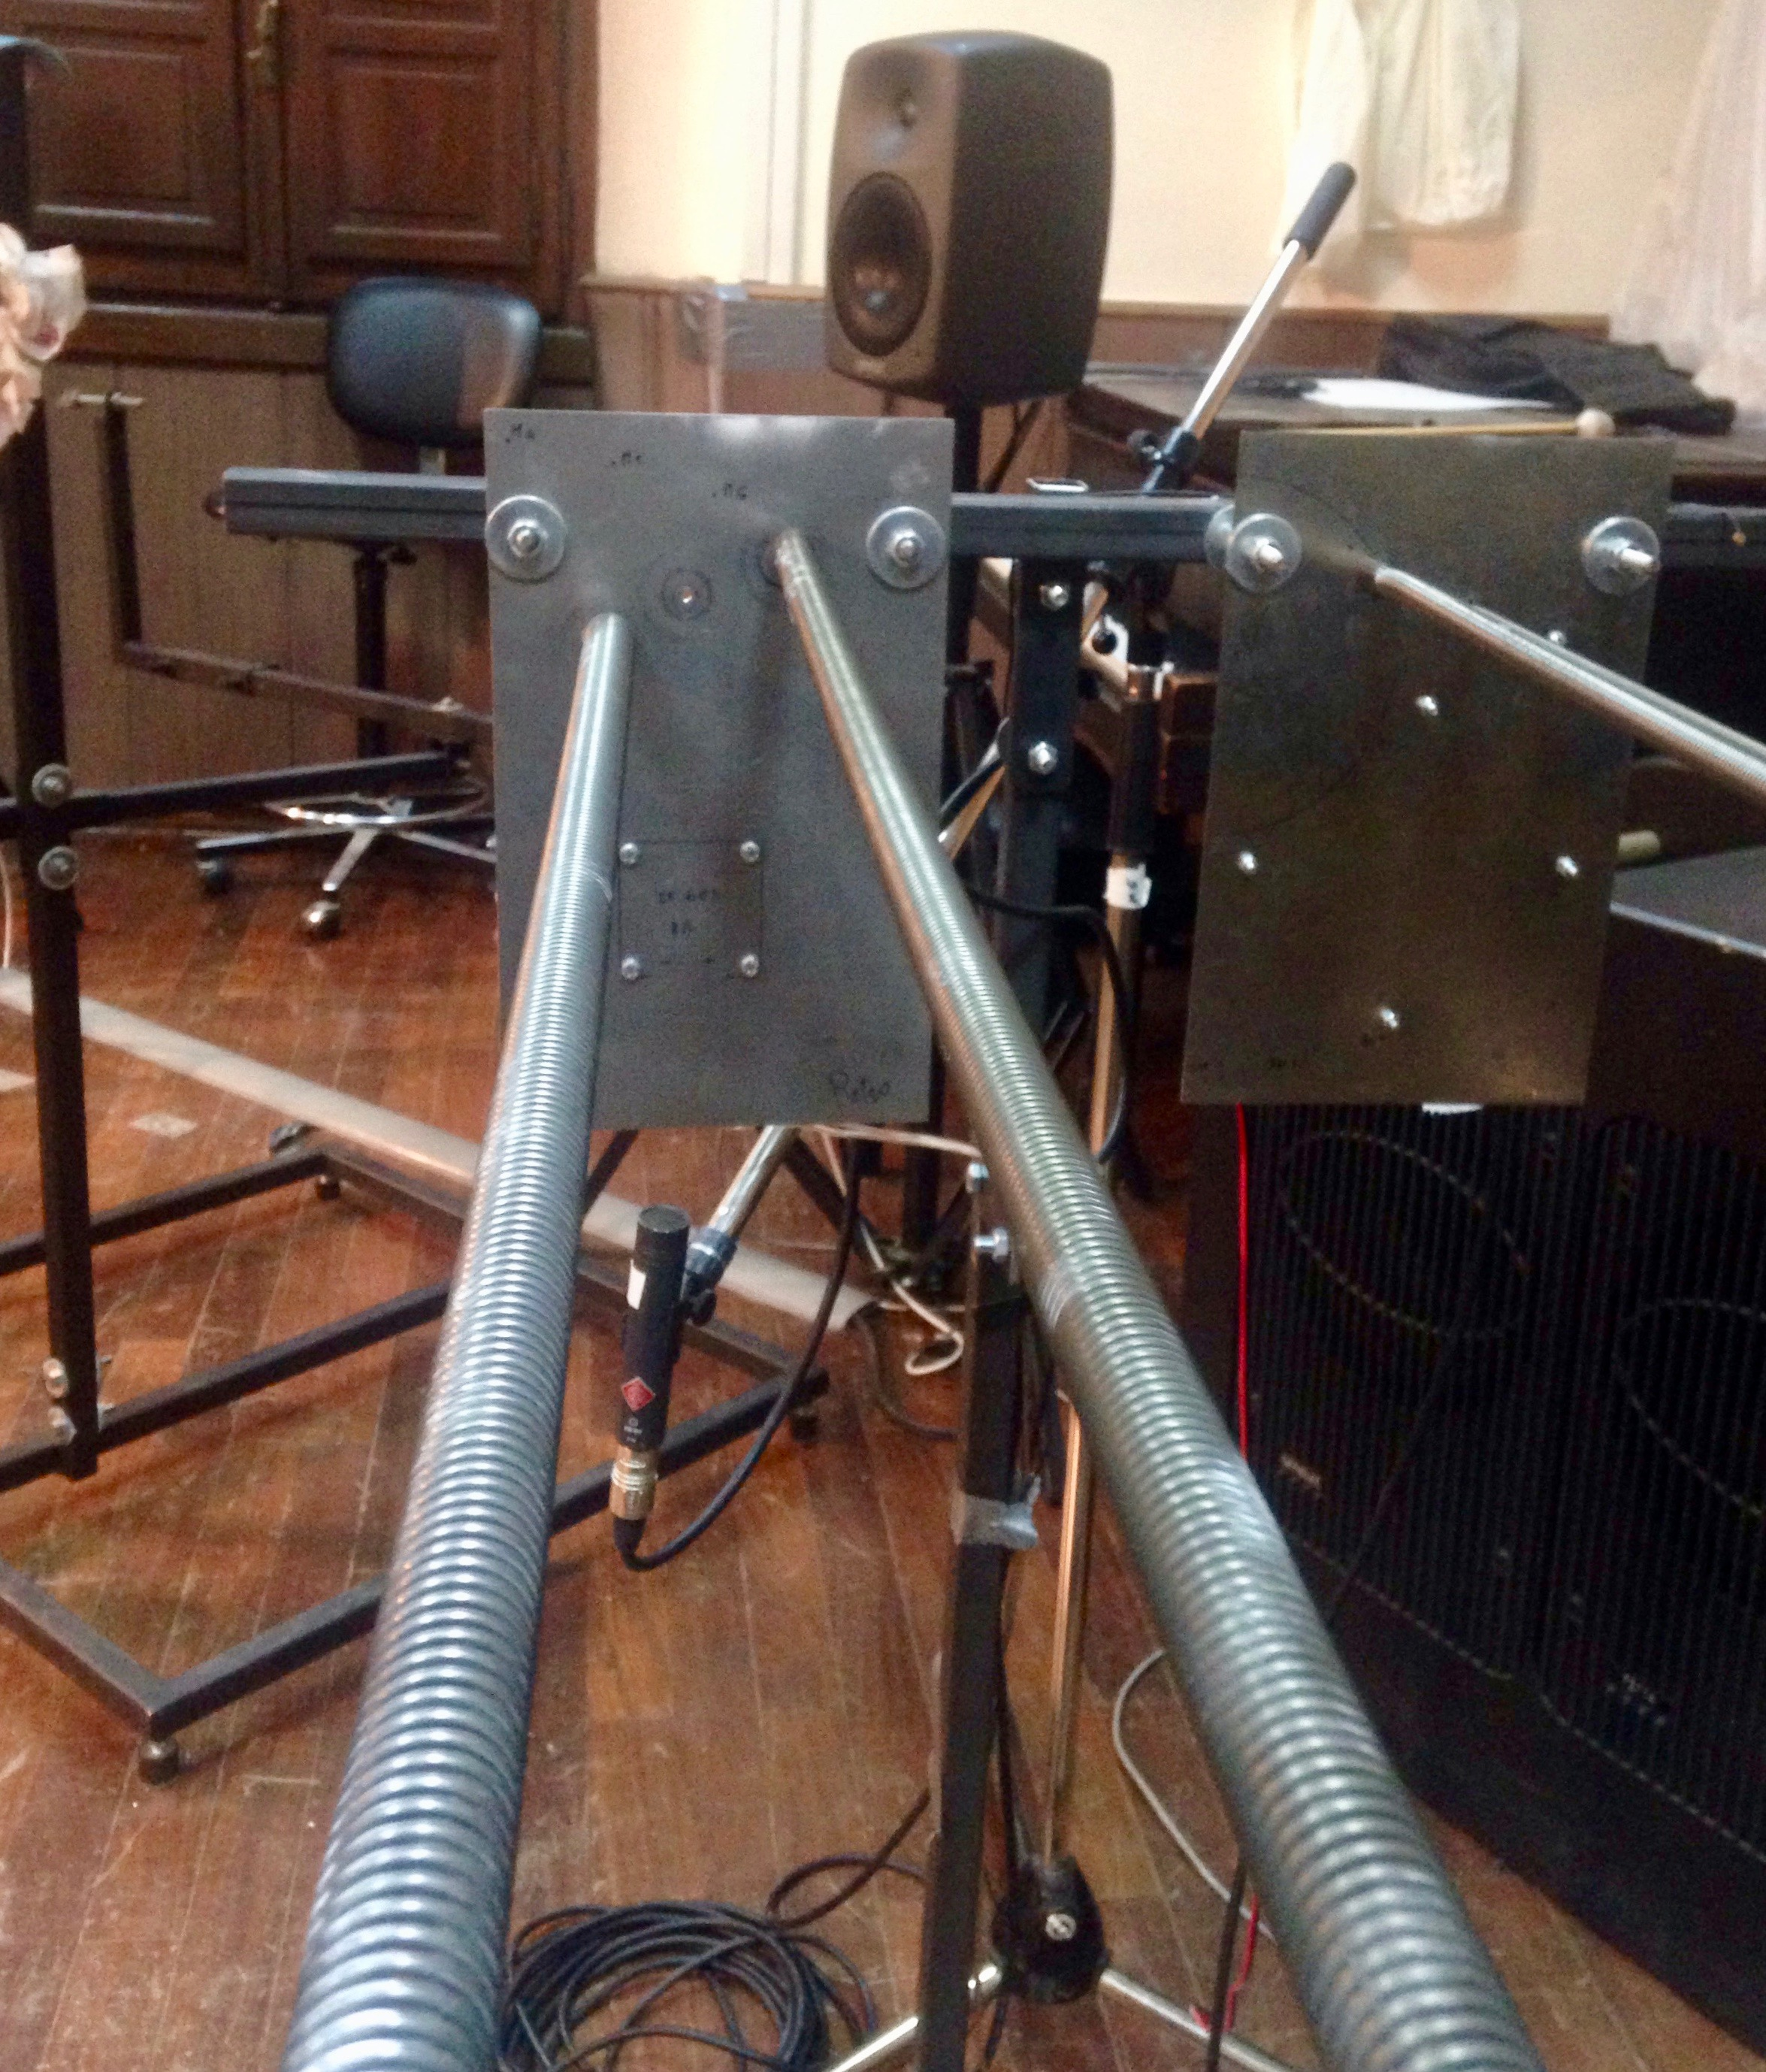
\includegraphics[width=.99\textwidth]{Spire2cc.jpg}
\caption{\textit{Sp.I.R.E.}, particolare della sezione più grave (Molla 5-4)}
\label{fig:molle4e5}
\end{center}
\end{figure}

Lentamente l'oggetto prendeva forma, il CRM mi fornì le lastre mancanti e il \textit{Mollificio Ciullo} \footnote{https://www.mollificiociullo.com} mi indirizzò nella scelta delle molle. Potei finalmente vedere, ma soprattutto sentire se tutte le mie idee portavano a qualcosa di reale. La svolta decisiva la ebbi durante il montaggio delle lastre, perché decisi di aggiungere una variante elettroacustica: degli attuatori. Gli attuatori (diffusori capaci di far risuonare il materiale sul quale vengono collocati) furono il tassello mancante. Come scrive Silvia Lanzalone in un suo saggio:

\begin{quotation}
\textit{La catena elettroacustica, nonostante il notevole perfezionamento tecnologico degli ultimi decenni verso l'accuratezza della riproduzione sonora, conferisce ancora al suono una trasformazione finale dovuta alla natura elettromeccanica dei suoi componenti, imponendovi dunque una deformazione che la rende decorrelata dal segnale che trasmette, nonché estranea ad esso dal punto di vista della sua identificazione percettiva nello spazio destinato alla sua diffusione}\footnote{Silvia Lanzalone \textit{Strumenti aumentati} in \textit{Acustica} UTET}.
\end{quotation}

Spesso, quasi sempre, il suono elettronico risulta svincolato dal suono acustico. L'aggiunta degli attuatori sulle lastre, fu, perciò, il passo vincente per ovviare a tale problematica. Agire come se stessi "aumentando" uno strumento acustico è stato il pensiero principale, anche se ancora trattavo l'opera come un \textit{oggetto sonoro}. Nelle prove, convogliai tutti i contributi elettronici (dalle elaborazioni alla sintesi) direttamente nei quattro attuatori,  trasformando così il mio oggetto sonoro in un vero e proprio \textit{strumento elettroacustico}: possibilità di rilascio "acustico" del suono e quindi interazione tra elementi acustici ed elettronici. 

Era nato lo \textit{Sp.I.R.E.}

%\begin{floatingfigure}{10cm}
%\mbox{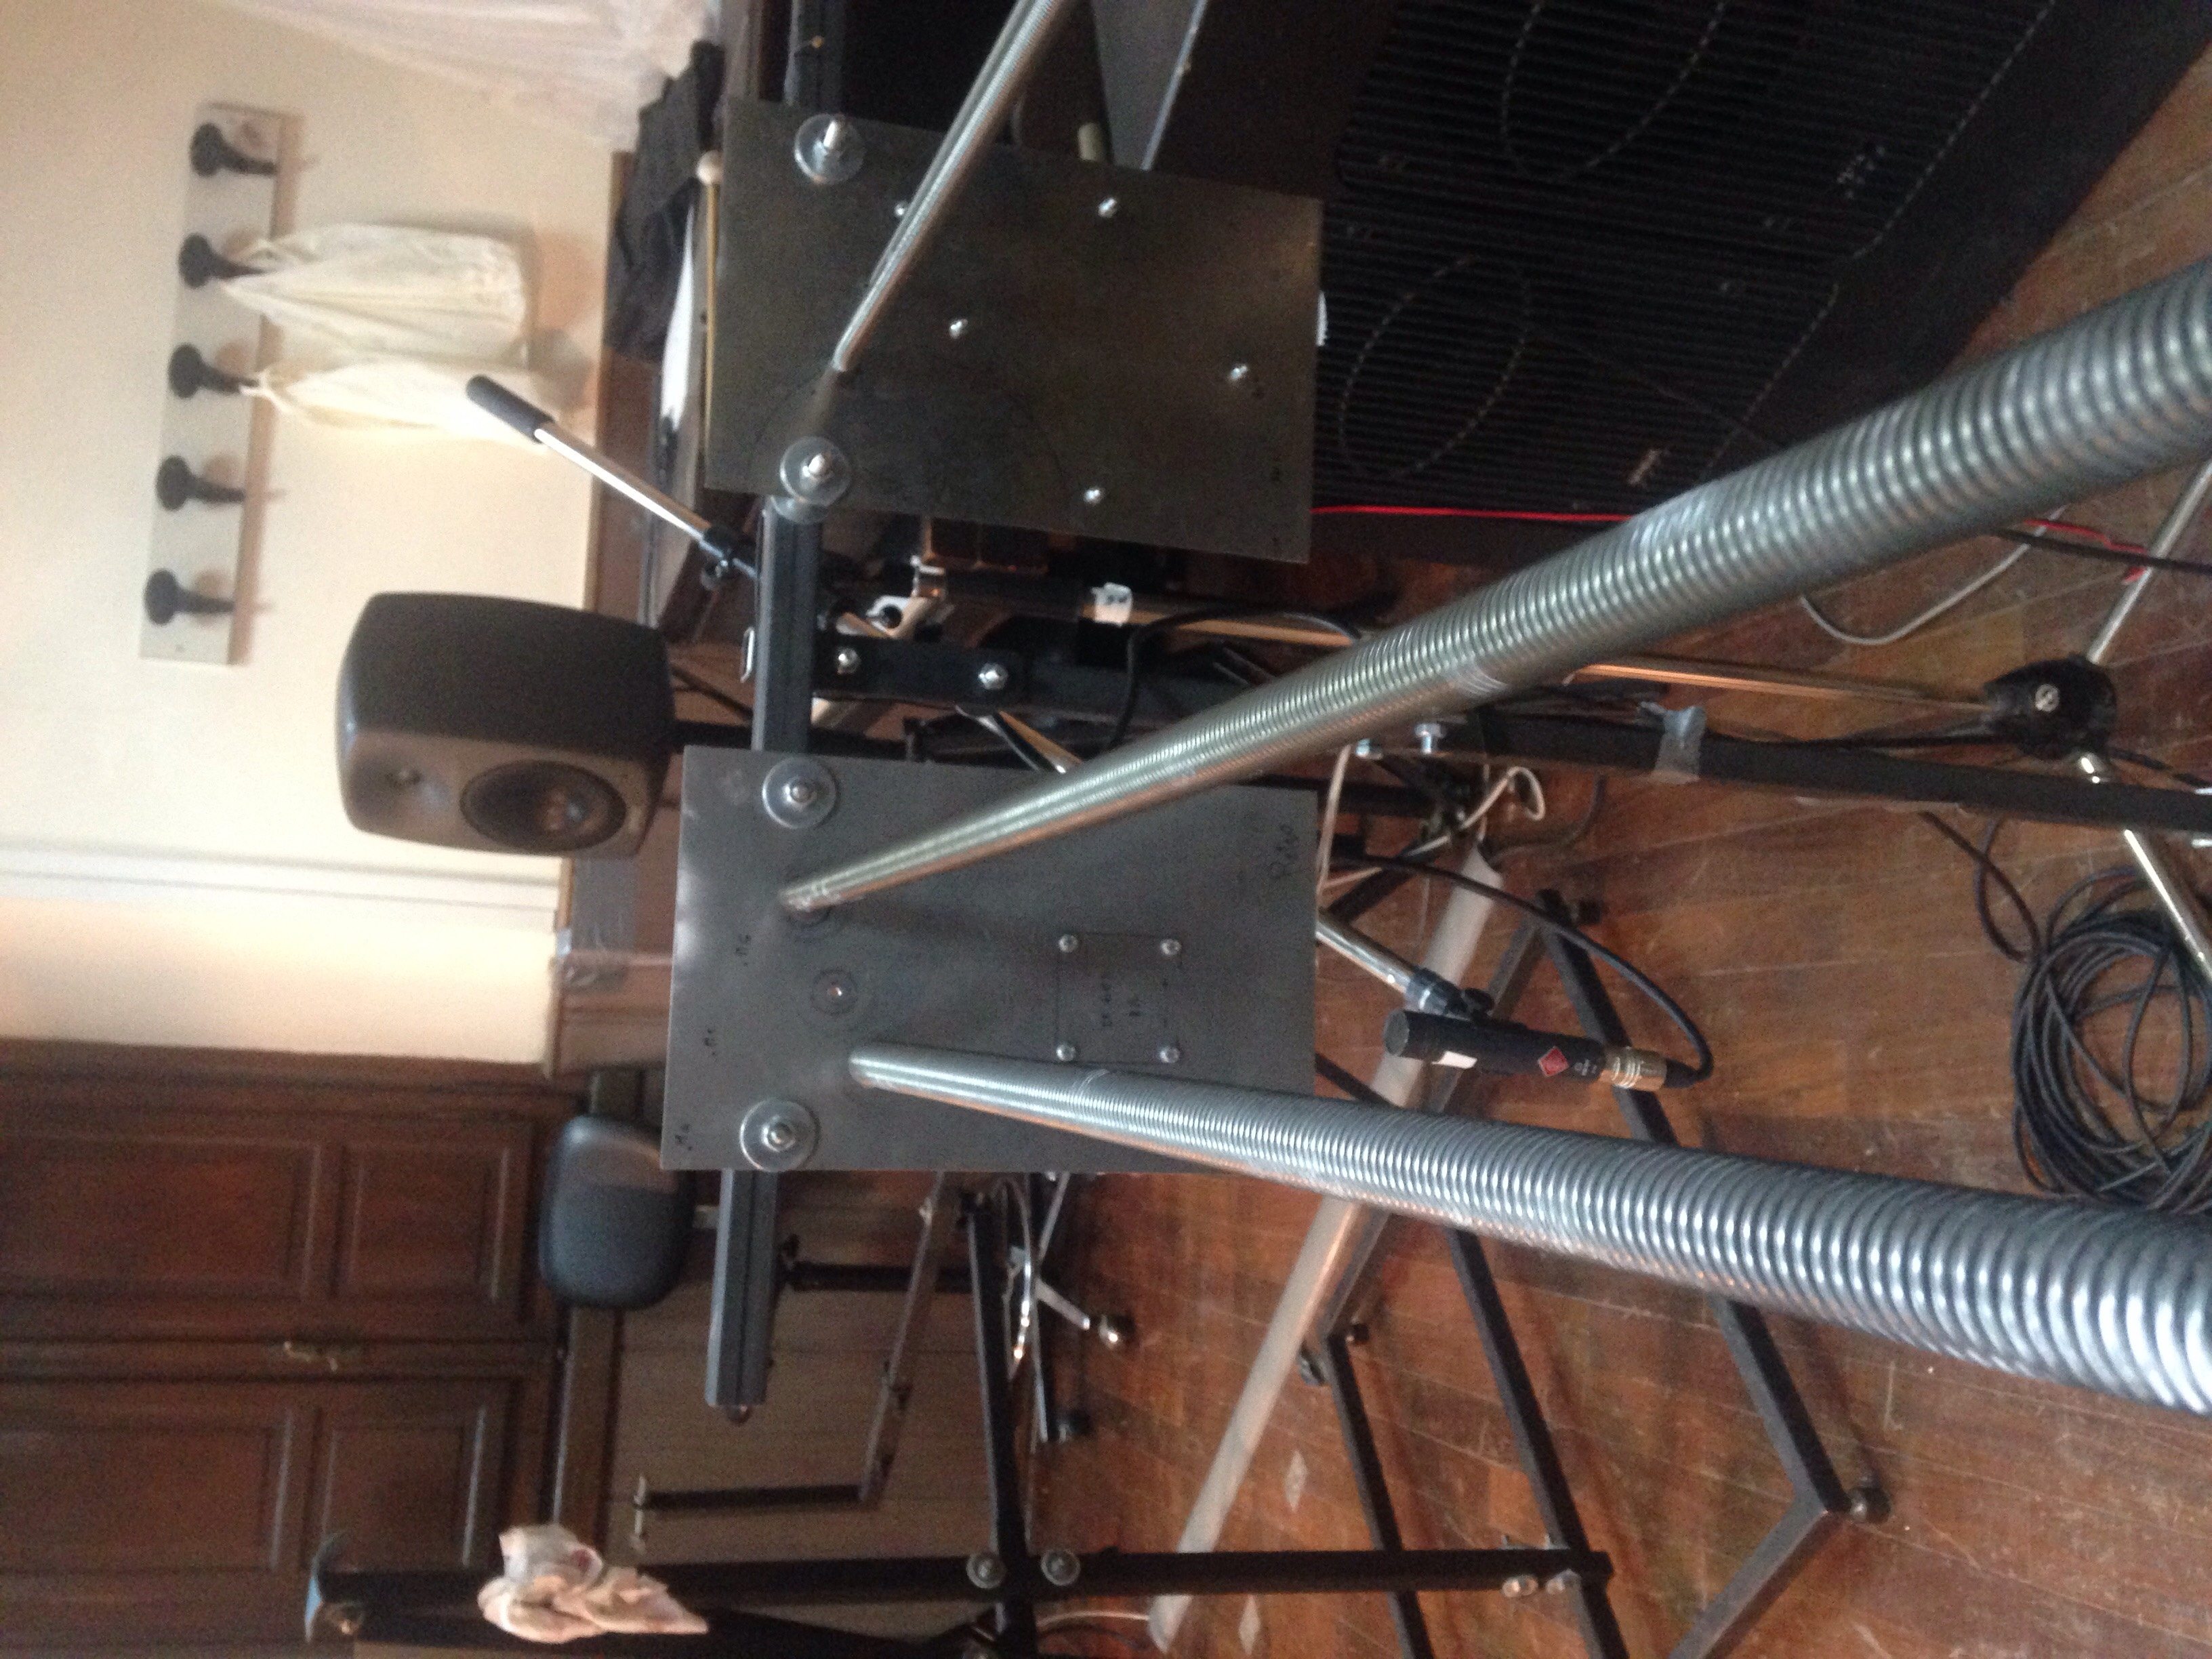
\epsfig{file=Spire2.jpg,width=8cm}}
%\small{\caption{\textit{particolare molle}}}
%\end{floatingfigure}



\textit{Sp.I.R.E.}, acronimo di \textit{Springs Installation Regulated \& Electrified}, fa riferimento alla fisicità del materiale che compone lo strumento. Ogni molla (\textit{spring}), infatti, è formata da \textit{spire} e il loro numero rende possibile, a seconda del materiale con il quale vengono eccitate, l'attivazione di armoniche e/o sub-armoniche. La parola \textit{electrified} indica la componente elettroacustica.

%\begin{floatingfigure}{10cm}
%\mbox{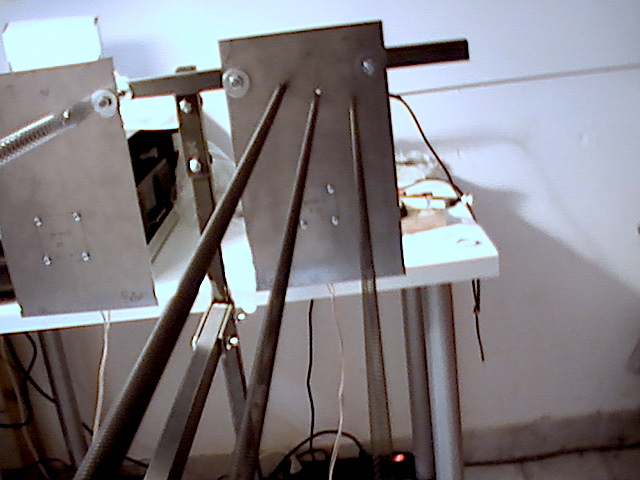
\epsfig{file=Prototipo2.jpg,width=8cm}}
%\small{\caption{\textit{particolare}}}
%\end{floatingfigure}

\begin{figure}[htbp]
\begin{center}
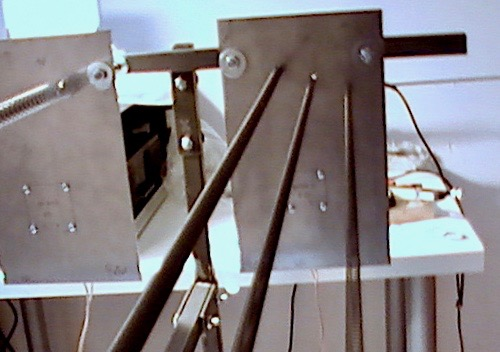
\includegraphics[width=.99\textwidth]{Prototipo2cc.jpg}
\caption{\textit{Sp.I.R.E.}, particolare della sezione più acuta (Molla 3-2-1)}
\label{fig:molle3e2e1}
\end{center}
\end{figure}

Questo esperimento è connesso allo studio di nuove identità formali relative alla natura dello strumento e alla realtà installativa dell'opera, che induce chi guarda e ascolta, a toccare la materia e ad incuriosirsi verso materiali come molle e placche di metallo, utilizzate per scopi lontani dall'utilizzo che se ne fa ogni giorno.

%************************************************

\section{Intenzioni espressive}

\epigraph{\textbf{spirare} v. intr. e tr. [lat. spirare «soffiare»; respirare; emanare»]"}
{\textit{Enciclopedia Treccani}}
La prima intenzione espressiva fu la creazione di uno strumento che avesse in sé le qualità del reverbero a molle e del reverbero a piastra. Il risultato fu esaltante: le molle sfregate con dita o archetti generavano un ambiente sonoro che le piastre amplificavano e modificavano, generando una coda piena di una propria identità timbrica.

Sp.i.r.e. è un progetto ambizioso che vuole, tra le altre cose, reinterpretare ed ampliare la visione di John Cage in Cartridge Music. La ricerca è basata, appunto, sul riuscire a rendere percepibili i suoni non udibili prodotti dallo strofinio delle molle o delle placche. Può essere considerato a tutti gli effetti uno strumento musicale, perché legato sia al mondo dei cordofoni che all'universo degli idiofoni (nel corso della performance verranno utilizzati sia archetti che battenti per percussioni).

\begin{figure}[htbp]
\begin{center}
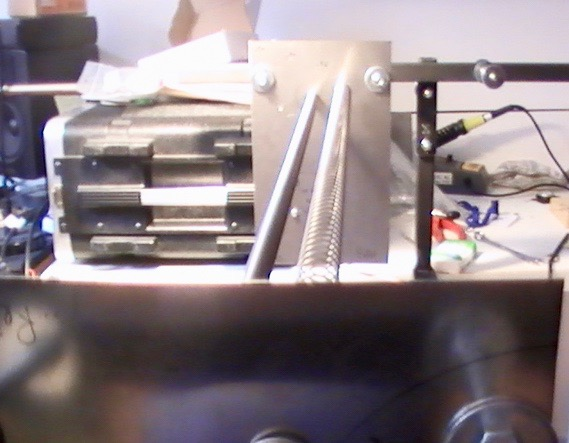
\includegraphics[width=.99\textwidth]{Prototipo3cc.jpg}
\caption{Foto scattata durante lavorazioni su Sp.I.R.E.}
\label{fig:lav}
\end{center}
\end{figure}

%************************************************

\section{Intenzioni estetiche}
Il progetto rappresenta il legame che c'è tra noi e il mondo che ci circonda: tutt'uno con la metropoli e con i fenomeni all'interno e all'esterno di essa\footnote{qui faccio riferimento di nuovo al concetto di fenomeno di Kandisky}.

Questa è l'identità di Sp.i.r.e., finalmente si tocca con mano la parte nascosta della materia, il lato più profondo di quello che vediamo attorno a noi. In unione ai suoni non udibili e all'invisibile, si scorge un richiamo verso una visione immaginifica che porta fino a dentro la nostra anatomia. Come se le spire della molla possono essere ricondotte ai ripiegamenti dell'intestino; come se, all'eccitazione di una molla, si riconduca la possibilità di produrre delle sub-armoniche e, in qualche modo, di avvicinarsi alle vibrazioni interne dell'anatomia umana.

La meccanica, l'elettronica e i suoni analogici, rendono possibile la creazione di un mondo nuovo. Vengono a formarsi più dimensioni d'ascolto e più dimensioni tattili, causate dalle diverse risposte d'eccitazioni del materiale. A questa dimensione d'ascolto si unisce la ripresa microfonica, che, nel caso di \textit{Vitres de Son}, sarà omnidirezionale e renderà possibile la riproduzione di tutto il panorama d'ascolto. Sp.i.r.e. \textit{respira} ed \textit{emana} il segnale elettroacustico in almeno due dimensioni d'ascolto:
\begin{enumerate}
\item{\textit{Analogica}, la risposta del materiale relativa ai suoni sintetici e al tocco umano}
\item{\textit{Elettrica ed elettronica}, che prende vita grazie ai suoni di sintesi diffusi dagli attuatori}
\end{enumerate}

L'insieme dei due fattori ha dato vita ad uno strumento che ingloba in sé, sia caratteristiche installative che performative. Una strana creature capace di suonare sia amplificata che in acustico grazie agli attuatori e al connubio fra placche e molle. La struttura è tutta \textit{suono}. Tendo a sottolineare che questo è ancora un primo prototipo e non mi fermerò prima di aver raggiunto determinati obbiettivi costruttivi e/o miglioramenti da applicare a breve sullo strumento. Come scrive Cage:

\begin{small}
\begin{quotation}
Decisi così di lavorare con qualunque strumento di produzione avessi incontrato e di tenere sempre un orecchio a terra, in cerca di un suono nuovo\footnote{John Cage, \textit{Confessioni di un compositore}}.
\end{quotation}
\end{small}

\clearpage

%************************************************

\section{Analisi spettrale}

Di seguito, l'analisi spettrale e lo spettrogramma della risposta all'eccitazione di ogni singola molla. 

\begin{figure}[htbp]
\begin{center}
\includegraphics[width=.99\textwidth]{MOLLA1.jpg}
\caption{Eccitazione \textit{Molla 5} tramite battente in legno.}
\label{fig:molla5legno}
\end{center}
\end{figure}

Sottolineo che l'eccitazione della molla è provocata colpendo al centro della molla. 
Negli studi fatti in questi mesi ho registrato un decadimento differente a seconda del battente utilizzato.
Si può notare come, sia l'attacco, che l'eccitazione delle armoniche è maggiore con questo battente. Ogni molla è soggetta ad un inviluppo e a un decadimento differente. Il decadimento è lungo circa 10 secondi, mentre l'attacco è molto veloce: tra 0,4 e 0,6 millisecondi. 
L'ultimo grafico rappresenta l'eccitazione di una molla con un battente in metallo (Fig. \ref{fig:battenti}, \emph{d}). 

%\begin{figure}[htbp]
%\begin{center}
%\includegraphics[width=.99\textwidth]{MOLLA2.jpg}
%\caption{Eccitazione \textit{Molla 4} tramite battente in legno.}
%\label{default}
%\end{center}
%\end{figure}
%
%\begin{figure}[htbp]
%\begin{center}
%\includegraphics[width=.99\textwidth]{MOLLA3.jpg}
%\caption{Eccitazione \textit{Molla 3} tramite battente in legno.}
%\label{default}
%\end{center}
%\end{figure}
%
%\begin{figure}[htbp]
%\begin{center}
%\includegraphics[width=.99\textwidth]{MOLLA4.jpg}
%\caption{Eccitazione \textit{Molla 2} tramite battente in legno.}
%\label{default}
%\end{center}
%\end{figure}
%
%
%
%\begin{figure}[htbp]
%\begin{center}
%\includegraphics[width=.99\textwidth]{MOLLA5.jpg}
%\caption{Eccitazione \textit{Molla 5} tramite battente in metallo.}
%\label{default}
%\end{center}
%\end{figure}

\begin{figure}
\centering
\subfloat[][\emph{Eccitazione \textit{Molla 2} tramite battente in legno.}]
   {\includegraphics[width=.75\textwidth]{MOLLA2.jpg}} \\
\subfloat[][\emph{Eccitazione \textit{Molla 3} tramite battente in legno.}]
   {\includegraphics[width=.75\textwidth]{MOLLA3.jpg}} \\
\subfloat[][\emph{Eccitazione \textit{Molla 4} tramite battente in legno.}]
   {\includegraphics[width=.75\textwidth]{MOLLA4.jpg}} \\
\subfloat[][\emph{Eccitazione \textit{Molla 5} tramite battente in metallo.}]
   {\includegraphics[width=.75\textwidth]{MOLLA5.jpg}}
\caption{analisi spettrale all'eccitazione di ogni singola molla}
\label{fig:battenti}
\end{figure}
